\documentclass[10pt]{article}

\def\Type{LessonDJ}
\def\TypeNum{Workshop Week 11} %Lesson #
\def\TypeTitle{Definite Integrals and Optimization } %Lesson Title
\def\Semester{Fall 2021} %Not Used 
\def\Course{MATH 1190}%Course number and name
\def\Targets{   \target{I1}, \target{I2}, \target{I3}, \target{A3} }

\usepackage{preambleDJ} 

%%%%%%%%%%%% BEGIN DOCUMENT %%%%%%%%%%%%%%%
%%%%%%%%%%%% BEGIN DOCUMENT %%%%%%%%%%%%%%%
%%%%%%%%%%%% BEGIN DOCUMENT %%%%%%%%%%%%%%%
%%%%%%%%%%%% BEGIN DOCUMENT %%%%%%%%%%%%%%%
%%%%%%%%%%%% BEGIN DOCUMENT %%%%%%%%%%%%%%%

\begin{document}
\pagestyle{otherpages}
\thispagestyle{firstpage}


\vs{.6}
\section{Estimating Definite Integrals and the Meaning of the Definite Integral}
\begin{enumerate}
    \item Consider the graph of $f(t)$\\% = -10t^3+10t+10$\\
    \mpageT{.4}{.6}{
       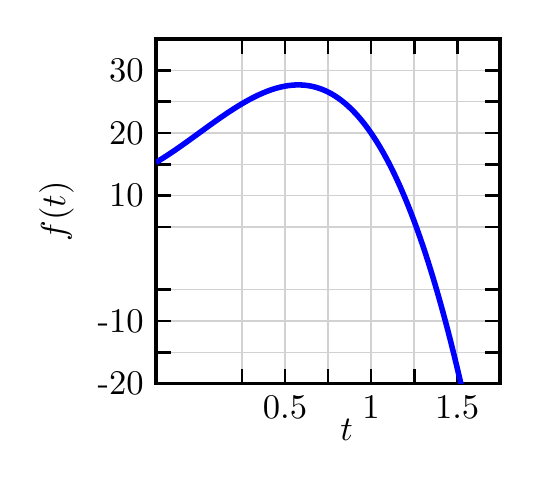
\begin{tikzpicture}[scale=1.25]
          \begin{axis}[
        %    axis y line = left,
            axis  line style= {line width = 1pt},
            xlabel={$t$},
            xtick       = {0.25,0.5,0.75,1,1.25,1.5,1.75},
            xticklabels = {,0.5,,1,,1.5},
            ytick       = {-20,-15,-10,-5,  5, 10, 15,20, 25,30,35},
             yticklabels = {-20,,-10,,,10,,20,,30,},
             major tick style = {black, thick},
            xlabel style={anchor=west},
                        ylabel={$f(t)$},
            ylabel style={anchor=south},
            samples     = 160,
            domain      = -.25:1.75,
            xmin = -0.25, xmax = 1.75,
            ymin = -20, ymax = 35,
            grid=both, grid style={gray!35},
            width=2in, height=2.in
          ]
          \addplot[domain=-0.25:1.75, blue, ultra thick, -] {20*(-x^3+x+1)};
        \end{axis}
    \end{tikzpicture}
    }{
%    \graphicsC{week11_spring.png}{3}
%    \begin{center}
%        
\includegraphics[scale = 0.5]{Fall 2025/1190 discussion/week11/images/week11_spring.png}
%    \end{center}
    \begin{enumerate}
        \item[(a)] Using $3$ rectangles, approximate the definite integral $\ds \int_0^{1.5} f(t) \;dt.$ Note, that there is more than one reasonable way to do this. And since this is an approximation,  you certainly won't get the exact answer!
    \end{enumerate}
    }
    \vs{1}
    \enum{
            \item[(b)]  $f(t)$ represents the velocity (in miles per hour) of a cyclist. In this context a positive velocity means the cyclist is traveling away from Newcomb Hall and a negative velocity means the cyclist is traveling towards Newcomb Hall.  We know that at time $t=0$ hours that the cyclist started 12 miles from Newcomb Hall.  What is the position of the cyclist at time $1.5$ hours?  
            }
            \end{enumerate}
    \newpage
    \section{Computing Definite Integrals}
    \enumR{
    \item Consider the function $f(x) = |x|.$\\
    \mpageT{.4}{.6}{
           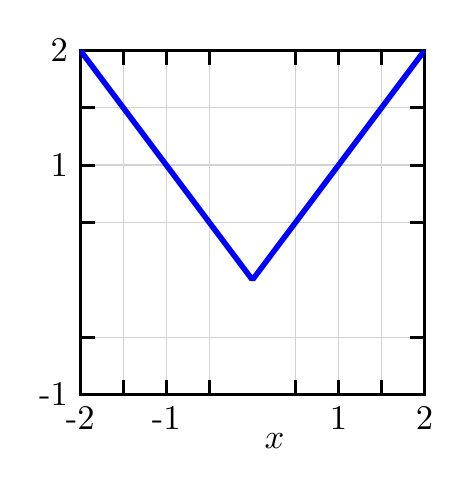
\begin{tikzpicture}[scale=1.25]
          \begin{axis}[
        %    axis y line = left,
            axis  line style= {line width = 1pt},
            xlabel={$x$},
            xtick       = {-2,-1.5,-1,-.5, .5,1,1.5,2},
            xticklabels = {-2,,-1,,,1,,2},
            ytick       = {-1,-.5,.5,1,1.5,2},
             yticklabels = {-1,,,1,,2},
             major tick style = {black, thick},
            xlabel style={anchor=west},
            ylabel style={anchor=south},
            samples     = 160,
            domain      = -1.25:1.15,
            xmin = -2, xmax = 2,
            ymin = -1, ymax = 2,
            grid=both, grid style={gray!35},
            width=2in, height=2.in
          ]
          \addplot[domain=-2:2, blue, ultra thick, -] {abs(x)};
        \end{axis}
    \end{tikzpicture}
    }{
    \begin{enumerate}
        \item[(a)] Compute $\ds \int_{-1}^1 f(x)dx.$
        \end{enumerate}
   }

        \mpageT{.4}{.6}{
                   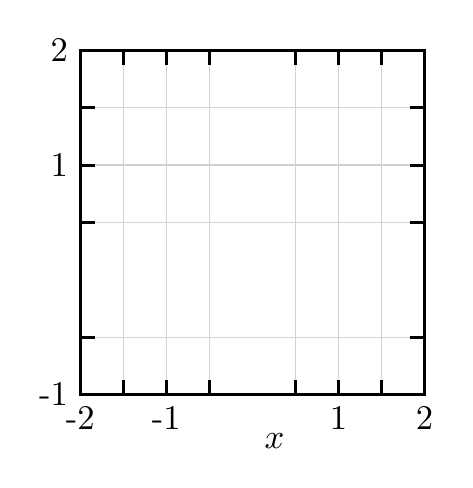
\begin{tikzpicture}[scale=1.25]
          \begin{axis}[
        %    axis y line = left,
            axis  line style= {line width = 1pt},
            xlabel={$x$},
            xtick       = {-2,-1.5,-1,-.5, .5,1,1.5,2},
            xticklabels = {-2,,-1,,,1,,2},
            ytick       = {-1,-.5,.5,1,1.5,2},
             yticklabels = {-1,,,1,,2},
             major tick style = {black, thick},
            xlabel style={anchor=west},
            ylabel style={anchor=south},
            samples     = 160,
            domain      = -1.25:1.15,
            xmin = -2, xmax = 2,
            ymin = -1, ymax = 2,
            grid=both, grid style={gray!35},
            width=2in, height=2.in
          ]
          %\addplot[domain=-2:2, blue, ultra thick, -] {abs(x)};
        \end{axis}
    \end{tikzpicture}
    }{       
     \begin{enumerate}
        \item[(b)] Compute $\ds \int_{-1}^1 f(x) + 1 ];dx.$ {\em Hint:} There are at least two reasonable approaches to this question. One approach might be to sketch the graph of $y=f(x)+1$.  An alternative approach might be to use the linearity property of definite integrals. There might be other reasonable approaches as well,
        \end{enumerate}
        }
        
           \mpageT{.4}{.6}{
                   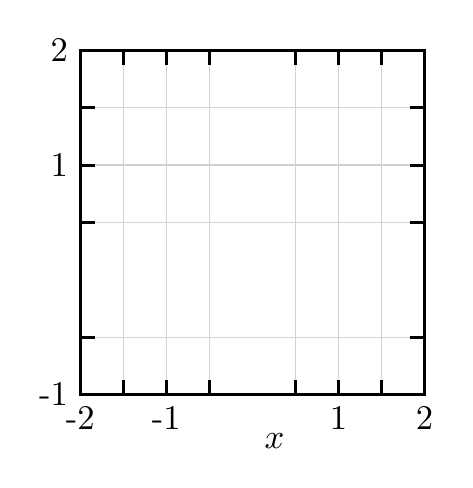
\begin{tikzpicture}[scale=1.25]
          \begin{axis}[
        %    axis y line = left,
            axis  line style= {line width = 1pt},
            xlabel={$x$},
            xtick       = {-2,-1.5,-1,-.5, .5,1,1.5,2},
            xticklabels = {-2,,-1,,,1,,2},
            ytick       = {-1,-.5,.5,1,1.5,2},
             yticklabels = {-1,,,1,,2},
             major tick style = {black, thick},
            xlabel style={anchor=west},
            ylabel style={anchor=south},
            samples     = 160,
            domain      = -1.25:1.15,
            xmin = -2, xmax = 2,
            ymin = -1, ymax = 2,
            grid=both, grid style={gray!35},
            width=2in, height=2.in
          ]
          %\addplot[domain=-2:2, blue, ultra thick, -] {abs(x)};
        \end{axis}
    \end{tikzpicture}
    }{    
        \begin{enumerate}
        \item[(c)] Compute $\ds \int_{-1}^1 f(x + 1)\;dx.$ {\em Hint:} It will be helpful to sketch the graph of $y=f(x+1)$.
    \end{enumerate}
    }
}
\newpage
\section{Properties of the Definite Integral}
    Consider the following graph of $f(x).$
\begin{center}
      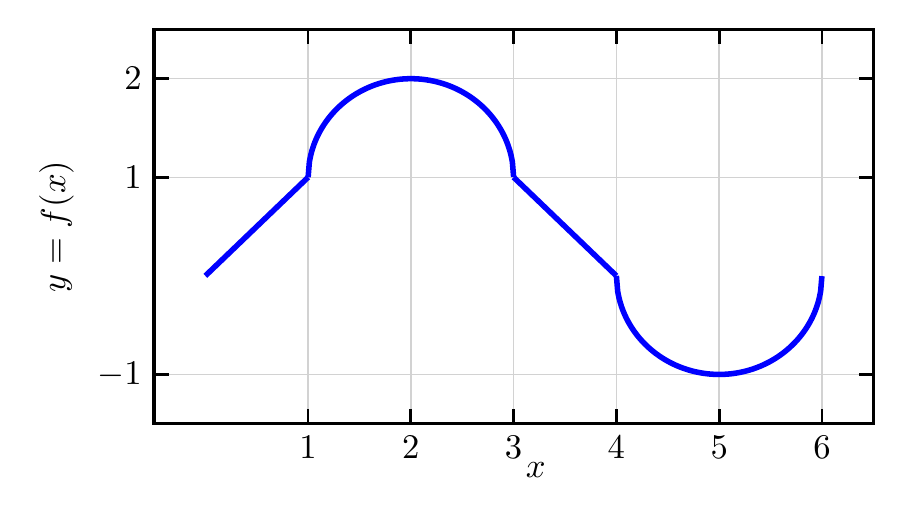
\begin{tikzpicture}[scale=1.25]
          \begin{axis}[
        %    axis y line = left,
            axis  line style= {line width = 1pt},
            xlabel={$x$},
            ylabel={$y=f(x)$},
            xtick       = {1,2,3,4,5,6},
            %xticklabels = {-2,,-1,,,1,,2},
            ytick       = {-1,1,2},
           %  yticklabels = {-1,,,1,,2},
             major tick style = {black, thick},
            xlabel style={anchor=west},
            ylabel style={anchor=south},
            samples     = 160,
            domain      = -1.25:1.15,
            xmin = -.5, xmax = 6.5,
            ymin = -1.5, ymax = 2.5,
            grid=both, grid style={gray!35},
            width=3.5in, height=2.2in
          ]
          \addplot[domain=0:1, blue, ultra thick, -] {x};
          \addplot[domain=1:3, blue, ultra thick, -] {sqrt(1-(x-2)^2)+1};
		\addplot[domain=3:4, blue, ultra thick, -] {4-x};
 		\addplot[domain=4:6, blue, ultra thick, -] {-sqrt(1-(x-5)^2)};
        \end{axis}
    \end{tikzpicture}
\end{center}
\enumR{
\item Compute the following integrals.
    \begin{enumerate}
        \item[(a)] Compute $\ds \int_0^6 f(x) \;dx$ exactly.
        \vs{.5}
        \item[(b)] Compute $\ds \int_2^4 f(x) \;dx$ exactly.
        \vs{.5}
        \item[(c)] Challenge question: Compute $\ds \int_0^6 |f(x)| dx.$
    \end{enumerate}
\item We don't know the graph of $g$, but suppose we do know $\dint_0^2 g(x)\,dx = 5$ and $\dint_2^4 g(x)\,dx=-4$. Compute the following integrals.
\begin{enumerate}
\item[(a)] $\displaystyle\int_0^2 (f(x)+g(x))\,dx$
\vs{.5}
\item[(b)] $\displaystyle\int_2^4 (f(x)+g(x))\,dx$
    \vs{.5}

\item[(c)] $\displaystyle\int_0^4 (f(x)+g(x))\,dx$
\vs{.5}

\item[(d)] $\displaystyle\int_4^0 5(f(x)+g(x))\,dx$
\end{enumerate}
    
}

\newpage
 \section{Optimization 1} 
\enumR{
     \item We want to construct a cylindrical can with a bottom but no top that will have a volume of 30 $cm^3$. What is the minimum surface area that such a cylinder can have? \\\\
     Note that the volume of a cylinder of height $h$ is $\ds V=\pi r^2\cdot h$, the surface area  of the side of the can is$SA_{side}=2\pi r\cdot h$ and the surface area of the bottom of the can is $SA_{bottom}=\pi r^2$
     }
     
     
     \newpage
     
     \section{Optimization 2}
     \enumR{
     \item We want to find two positive numbers, $a$ and $b,$ whose product is $250,$ and which minimizes $F=a + 10b.$
}
 \newpage
\section{Anti-derivatives}
\enumR{
    \item Compute
    \begin{enumerate}
   %     \item $\ds \int e^x \,dx=$
        \item $\ds \int 3^x \,dx=$ 
        \item $\ds \int \frac{1}{x^2} \,dx =$ 
        \item $\ds \int \frac{10}{x} \,dx =$
        \item $\ds \int 2^5 \,dx =$ 
       % \item $\ds \int \log(2) \,dx =$ 
        \item $\ds \int \frac23x^4 \,dx =$
        \item $\ds \int \sqrt{x^3} \,dx =$
    \end{enumerate}

    \item Compute 
    \begin{enumerate}
        \item $\ds \int (x^4 - x^3 + x^2)(x^2 + 1)\,dx.$
        \item $\ds \int   \frac{x^3+ 2x + 10x^9}{x^2}\,dx.$
    \end{enumerate}    



}
\end{document}